% Options for packages loaded elsewhere
\PassOptionsToPackage{unicode}{hyperref}
\PassOptionsToPackage{hyphens}{url}
%
\documentclass[
]{article}
\title{Exploring the seasonal variation in electric vehicle charging in
New Zealand}
\author{Pablo Paulsen}
\date{18/02/2022}

\usepackage{amsmath,amssymb}
\usepackage{lmodern}
\usepackage{iftex}
\ifPDFTeX
  \usepackage[T1]{fontenc}
  \usepackage[utf8]{inputenc}
  \usepackage{textcomp} % provide euro and other symbols
\else % if luatex or xetex
  \usepackage{unicode-math}
  \defaultfontfeatures{Scale=MatchLowercase}
  \defaultfontfeatures[\rmfamily]{Ligatures=TeX,Scale=1}
\fi
% Use upquote if available, for straight quotes in verbatim environments
\IfFileExists{upquote.sty}{\usepackage{upquote}}{}
\IfFileExists{microtype.sty}{% use microtype if available
  \usepackage[]{microtype}
  \UseMicrotypeSet[protrusion]{basicmath} % disable protrusion for tt fonts
}{}
\makeatletter
\@ifundefined{KOMAClassName}{% if non-KOMA class
  \IfFileExists{parskip.sty}{%
    \usepackage{parskip}
  }{% else
    \setlength{\parindent}{0pt}
    \setlength{\parskip}{6pt plus 2pt minus 1pt}}
}{% if KOMA class
  \KOMAoptions{parskip=half}}
\makeatother
\usepackage{xcolor}
\IfFileExists{xurl.sty}{\usepackage{xurl}}{} % add URL line breaks if available
\IfFileExists{bookmark.sty}{\usepackage{bookmark}}{\usepackage{hyperref}}
\hypersetup{
  pdftitle={Exploring the seasonal variation in electric vehicle charging in New Zealand},
  pdfauthor={Pablo Paulsen},
  hidelinks,
  pdfcreator={LaTeX via pandoc}}
\urlstyle{same} % disable monospaced font for URLs
\usepackage[margin=1in]{geometry}
\usepackage{longtable,booktabs,array}
\usepackage{calc} % for calculating minipage widths
% Correct order of tables after \paragraph or \subparagraph
\usepackage{etoolbox}
\makeatletter
\patchcmd\longtable{\par}{\if@noskipsec\mbox{}\fi\par}{}{}
\makeatother
% Allow footnotes in longtable head/foot
\IfFileExists{footnotehyper.sty}{\usepackage{footnotehyper}}{\usepackage{footnote}}
\makesavenoteenv{longtable}
\usepackage{graphicx}
\makeatletter
\def\maxwidth{\ifdim\Gin@nat@width>\linewidth\linewidth\else\Gin@nat@width\fi}
\def\maxheight{\ifdim\Gin@nat@height>\textheight\textheight\else\Gin@nat@height\fi}
\makeatother
% Scale images if necessary, so that they will not overflow the page
% margins by default, and it is still possible to overwrite the defaults
% using explicit options in \includegraphics[width, height, ...]{}
\setkeys{Gin}{width=\maxwidth,height=\maxheight,keepaspectratio}
% Set default figure placement to htbp
\makeatletter
\def\fps@figure{htbp}
\makeatother
\setlength{\emergencystretch}{3em} % prevent overfull lines
\providecommand{\tightlist}{%
  \setlength{\itemsep}{0pt}\setlength{\parskip}{0pt}}
\setcounter{secnumdepth}{-\maxdimen} % remove section numbering
\usepackage{float}
\floatplacement{figure}{H}
\usepackage{comment}
\ifLuaTeX
  \usepackage{selnolig}  % disable illegal ligatures
\fi

\begin{document}
\maketitle

\begin{equation}
\label{eq1}
E_{m,R} = \eta_{m,R} \times d_{m,R}
\end{equation}

\ref{eq1}

\hypertarget{data-exploration}{%
\subsection{Data Exploration}\label{data-exploration}}

\hypertarget{flip-the-fleet-data-exploration}{%
\subsubsection{Flip the Fleet Data
Exploration}\label{flip-the-fleet-data-exploration}}

Distance traveled and vehicle energy efficiency (km/kWh) by month, as
well as the region of the vehicle was collected from the on-board
computers of 1259 electric vehicles (EV) between 2017 and 2021 by Flip
the Fleet \cite{ftf}.

Energy economy (Wh/km) was calculated as the inverse of efficiency
(km/kWh). Energy economy will be used instead of efficiency in the
modelling in this work for reasons that will become apparent later in
the analysis.

A monthly weighted average energy economy was calculated for the whole
of New Zealand and then for each region. The monthly averages were
weighted using the distance traveled to give more weighting to vehicles
with higher km traveled in that month. This was done using the formula

\[\bar{x} = \frac{\sum_{i}^{n} (d_i\times x_i)}{\left(\sum_{i}^{n} d_i\right)\times n}\]

\begin{figure}
\centering
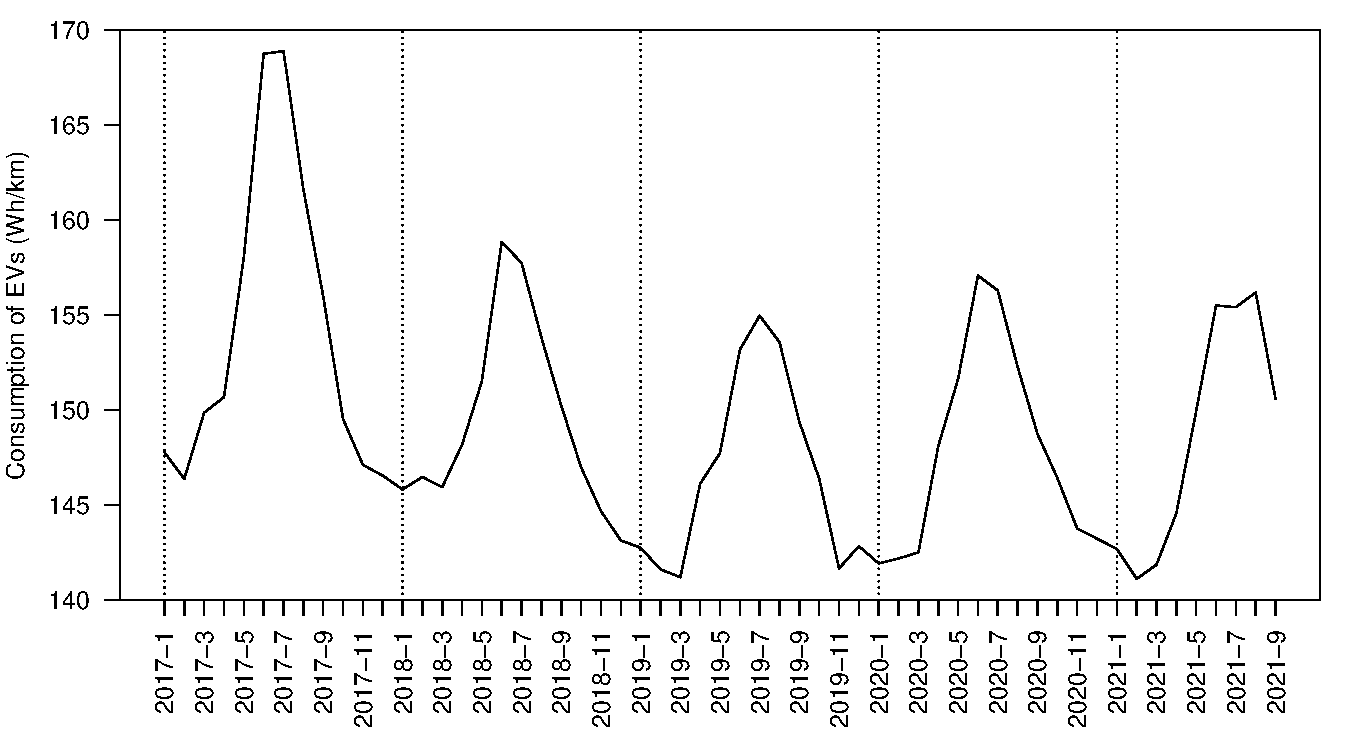
\includegraphics{final_report_files/figure-latex/consum_plot-1.pdf}
\caption{National monthly average energy economy of Flip the Fleet
vehicles\label{fig:consum_plot}}
\end{figure}

Figure \ref{fig:consum_plot} shows there is a clear seasonal trend in
the national monthly average energy economy of Flip the Fleets vehicles.

A time series decomposition is used to isolate the seasonal trend in
energy economy from the overall trend. This can be done for all regions
of NZ combined and also for each region individually.

\begin{figure}
\centering
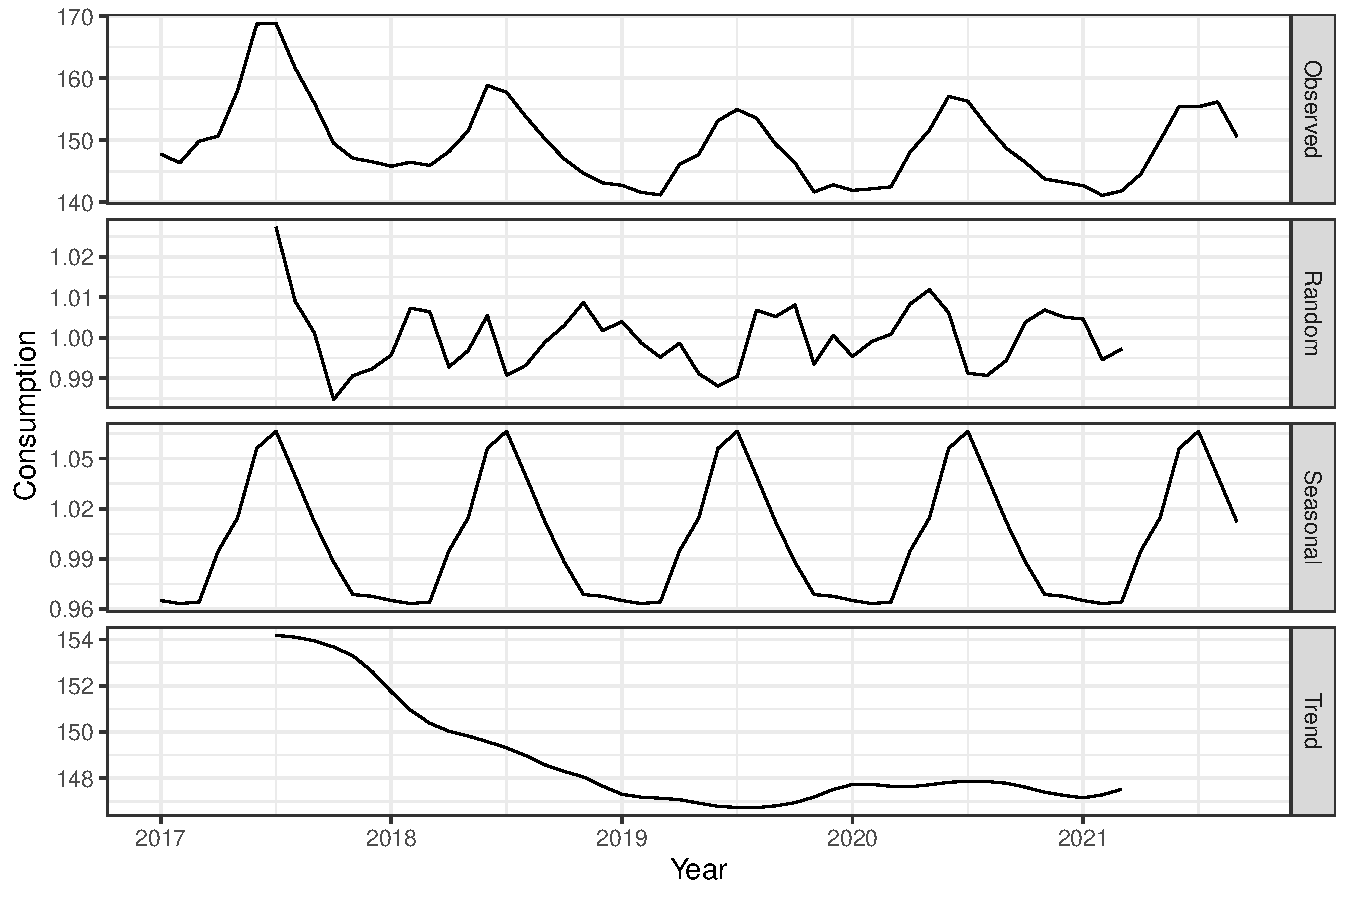
\includegraphics{final_report_files/figure-latex/consum_decomp_plot-1.pdf}
\caption{Multiplicative time series decomposition of Flip the Fleet
average energy economy for all of NZ\label{fig:consum_decomp_plot}}
\end{figure}

\begin{figure}
\centering
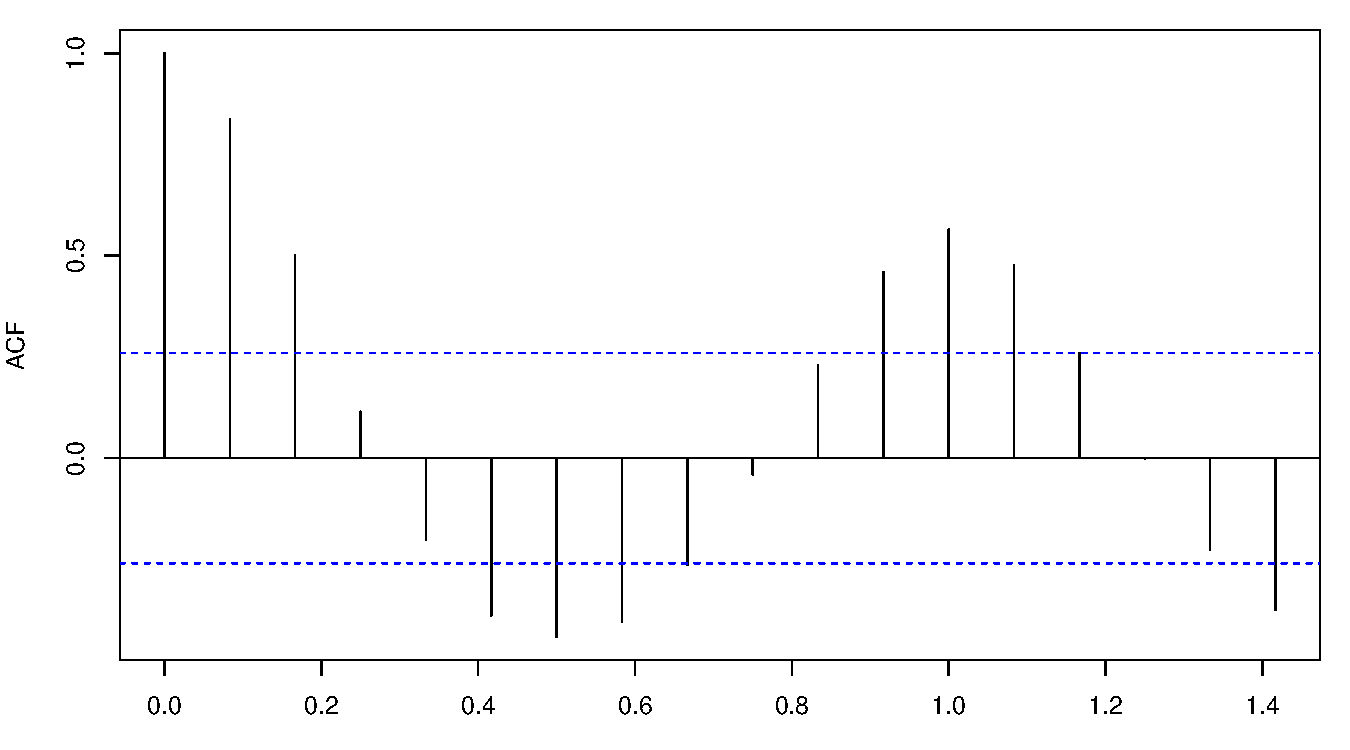
\includegraphics{final_report_files/figure-latex/acf_consum-1.pdf}
\caption{Autocorrelation plot of Flip the Fleet average energy economy
for all of NZ\label{fig:acf_consum}}
\end{figure}

The time series decomposition (Figure \ref{fig:consum_decomp_plot})
shows a very clear seasonal trend. The autocorrelation plot (Figure
\ref{fig:acf_consum}) shows that this yearly trend is significant. This
seasonal trend goes from 0.96 times the mean energy economy in February
to 1.07 times the mean energy economy in July, a peak to peak difference
of 10.7\%.

Past research shows that a majority of the seasonal variation in EV
efficiency is due to cabin temperature control\cite{ev_range}. This
would suggest that EV energy economy is correlated with heating degree
days. To test this hypothesis, as NZ weather differs significantly by
region, we must limit the comparison to a single region and compare it
to that regions weather at the same period of time.

In order to do this, hourly weather data from 2017 to 2021 was collected
from the NIWA National Climate Database for 14 regions around New
Zealand that best correspond to the regions of the Flip the Fleet
vehicles. Using the regional hourly temperatures, monthly heating degree
days (HDD) and cooling degree days (CDD) were imputed using base
temperatures of 16\(^\circ\)C and 22\(^\circ\)C respectively. These base
temperatures were selected to represent the range of comfortable
temperatures for most people. Monthly average temperature were also
calculated.

The HDD and CDD was then divided by the length of the month to determine
to average heating/cooling degrees days per day for the month. This is
so that when comparing to other statistics, such as efficiency that are
averaged out rather than summed, there is less bias.

The calculated monthly weather statistics by region was then compared to
the monthly EV data based on the regions of vehicle. This assumes that
most vehicles stay in their own region for a majority of the time.

\begin{figure}
\centering
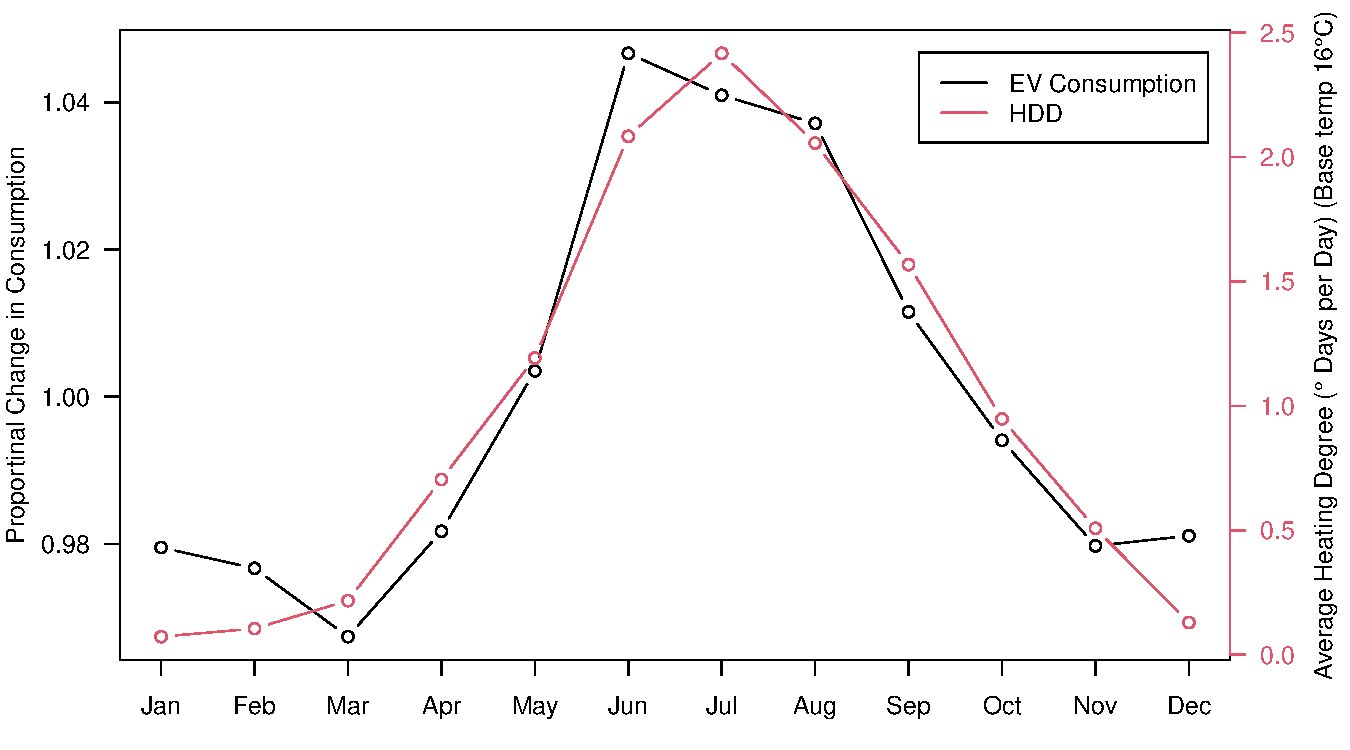
\includegraphics{final_report_files/figure-latex/consum_HDD_plot-1.pdf}
\caption{Auckland seasonal HDD and EV energy economy
decompostions\label{fig:consum_HDD_plot}}
\end{figure}

Auckland is used as an example to compare correlation between HDD and
energy economy as it has the largest amount of data and is of most
interest to Vector. Within Auckland, Figure \ref{fig:consum_HDD_plot}
shows very clearly that HDD and energy economy of EVs are highly
correlated. There is a slight increase in energy economy in January and
February and it can be questioned if that is due to AC usage which would
decrease range \cite{ev_range} or other factors such as holiday travel,
often involving highway driving which EVs are generally less efficient
at \cite{ev_highway}. This effect is not obvious in the overall trend
for NZ, so due to the fact that Auckland for the most part is a warmer
climate than the rest of NZ.

\begin{figure}
\centering
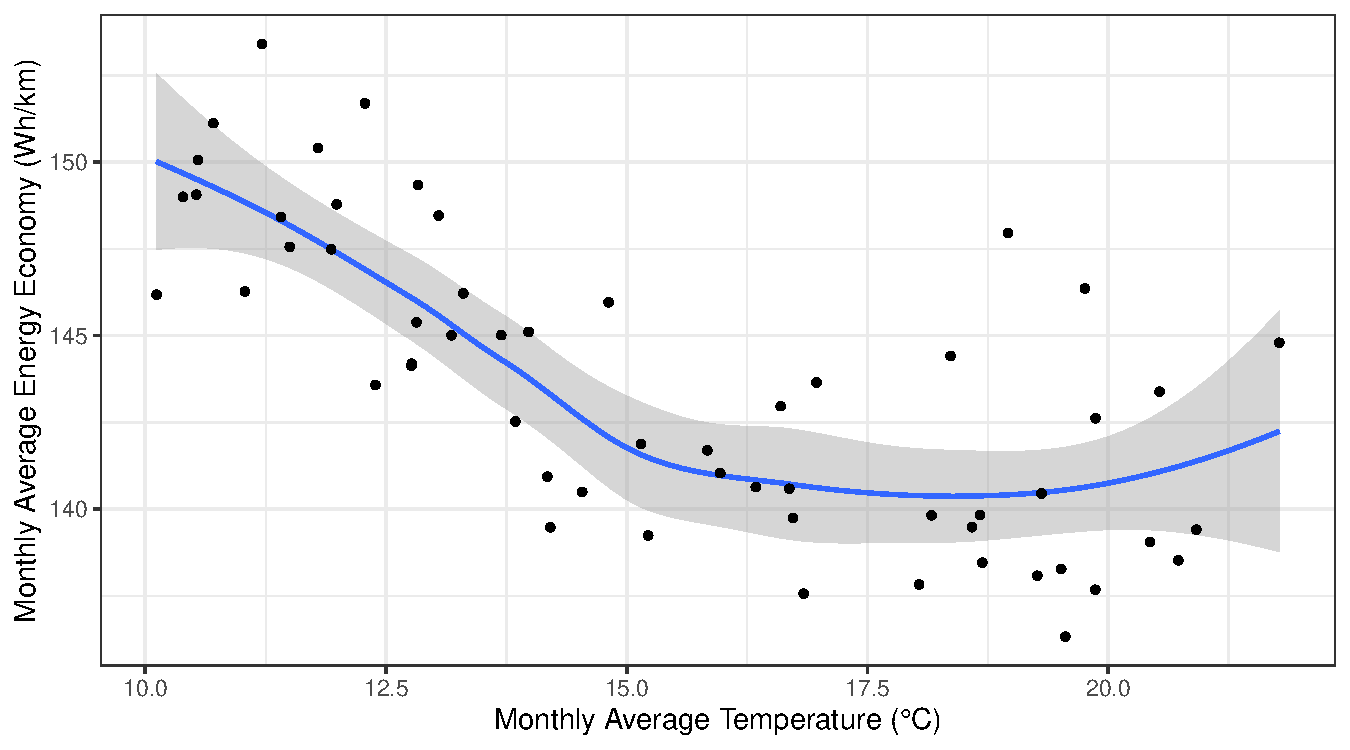
\includegraphics{final_report_files/figure-latex/temp_consum_plot-1.pdf}
\caption{Auckland monthly average energy economy by avg
temperature\label{fig:temp_consum_plot}}
\end{figure}

Further exploring the relation between energy economy and weather in
Auckland, Figure \ref{fig:temp_consum_plot} shows a decreasing energy
economy up to around a monthly average temperature of 17.5°C. However,
increasing monthly average temperature past this, there appears to be a
trend towards increasing EV energy economy. As stated previously,
research \cite{ev_range} suggested AC also increases energy economy of
EVs. This suggests it may be worth including both cooling degree days
and heating degree days in the analysis. This could also be useful to
explain the points well above the trend line that may be from a month
where there was both cold and warm days contributing to a high usage of
cabin temperature control, increasing energy economy, but average
temperature would not be able to show this.

\hypertarget{nz-vkt-data-exploration}{%
\subsubsection{NZ VKT Data Exploration}\label{nz-vkt-data-exploration}}

To determine the season impacts of EV charging on our electricity grid
we also need to explore seasonality in driving patterns. A number of
data sets were considered including fuel usage and vehicle kilometers
traveled (VKT) data.

To explore the seasonal trend in fuel usage in NZ, fuel trade data
\cite{fuel_trade} from the Ministry of Business, Innovation and
Employment (MBIE) is used. This data set includes quarterly fuel usage
data broken down by fuel type and sector. This allows the isolation of
petrol usage in domestic land transport, which should provide an
estimate of the fuel usage by light passenger vehicles. Fuel trade data
from 2020 was excluded as lockdowns were not an accurate representation
of the general driving patterns of the NZ population.

\begin{figure}
\centering
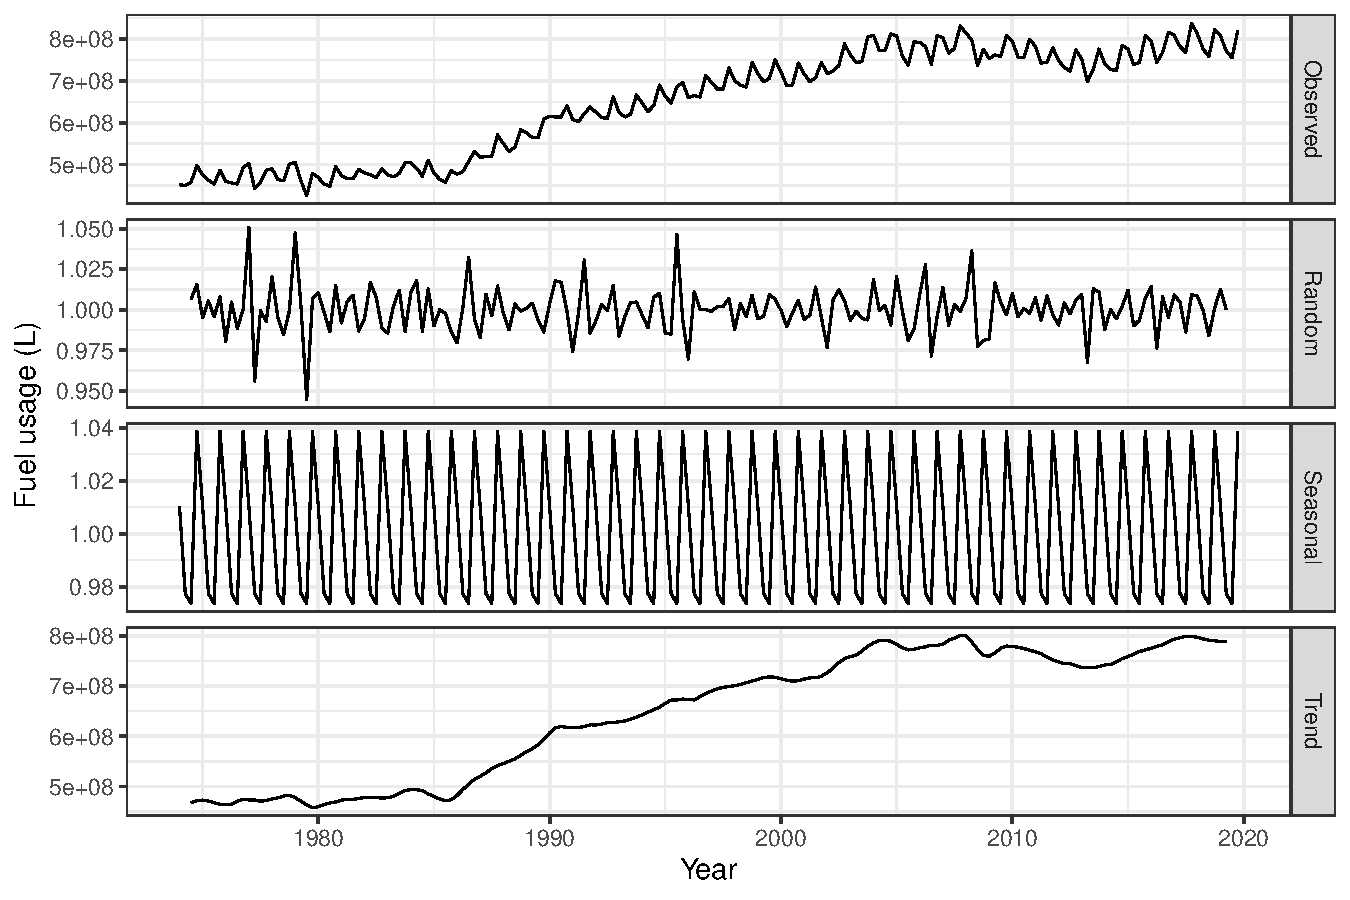
\includegraphics{final_report_files/figure-latex/petrol_ts-1.pdf}
\caption{Multiplicative time series decomposition of petrol usage in
domestic land transport\label{fig:petrol_ts}}
\end{figure}

Figure \ref{fig:petrol_ts} time series decomposition shows a seasonal
trend in petrol usage, however, it is of relatively small magnitude
compared to the random variations suggesting this trend may not be
significant.

\begin{figure}
\centering
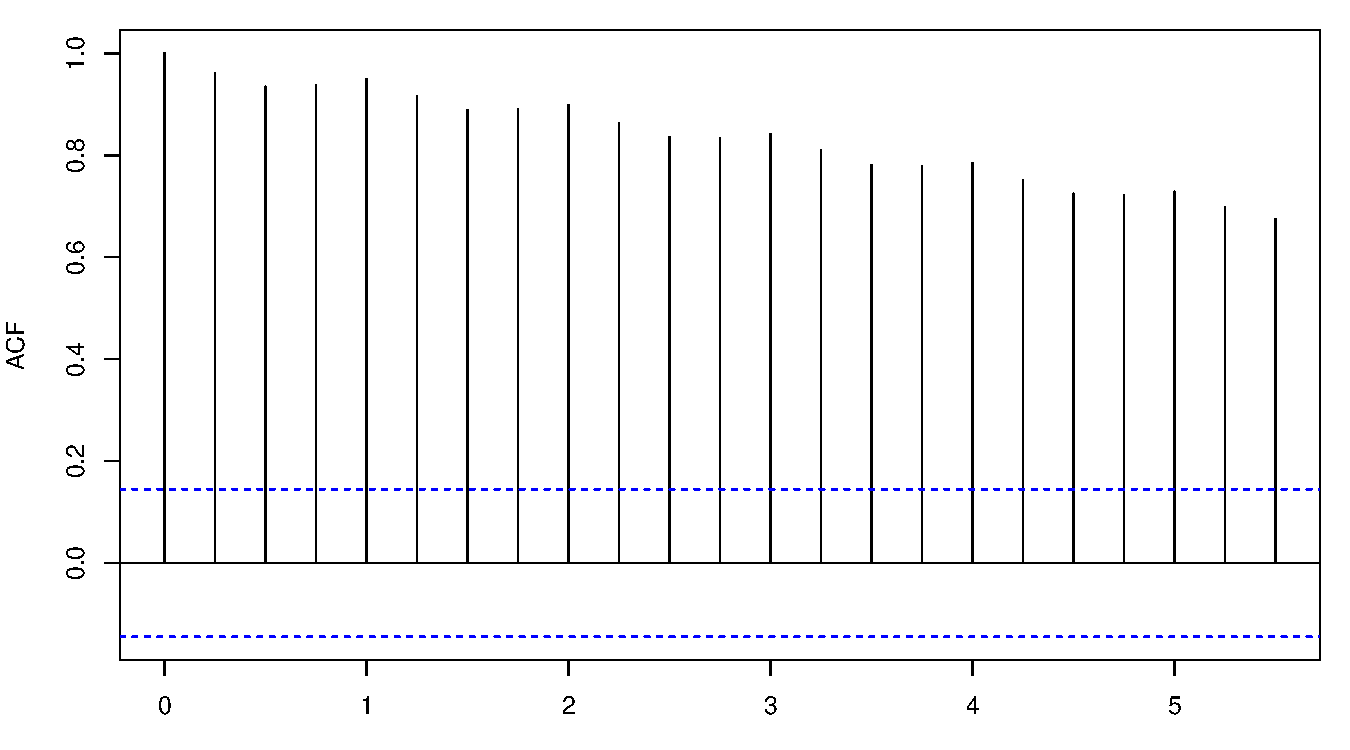
\includegraphics{final_report_files/figure-latex/acf_petrol-1.pdf}
\caption{Autocorrelation of petrol usage in domestic land
transport\label{fig:acf_petrol}}
\end{figure}

The autocorrelation plot (figure \ref{fig:acf_petrol}) suggest that
there might be a slight trend in petrol usage however it does not appear
to be of much significance.

Fuel trade data can be compared to the VKT data from the Ministry of
Transport. VKT data including quarterly data of 10 regions plus one
``other'' region was given by Haobo Wang from the Ministry of Transport
for use in this project. Further yearly data for VKT of the ``other''
regions, the vehicle fuel type and vehicle type was collected from the
publicly available fleet statistics page on Ministry of Transport's
website. The quarterly VKT data was then multiplied by the proportion of
VKT that was attributed to light passenger vehicles in that year.

\begin{figure}
\centering
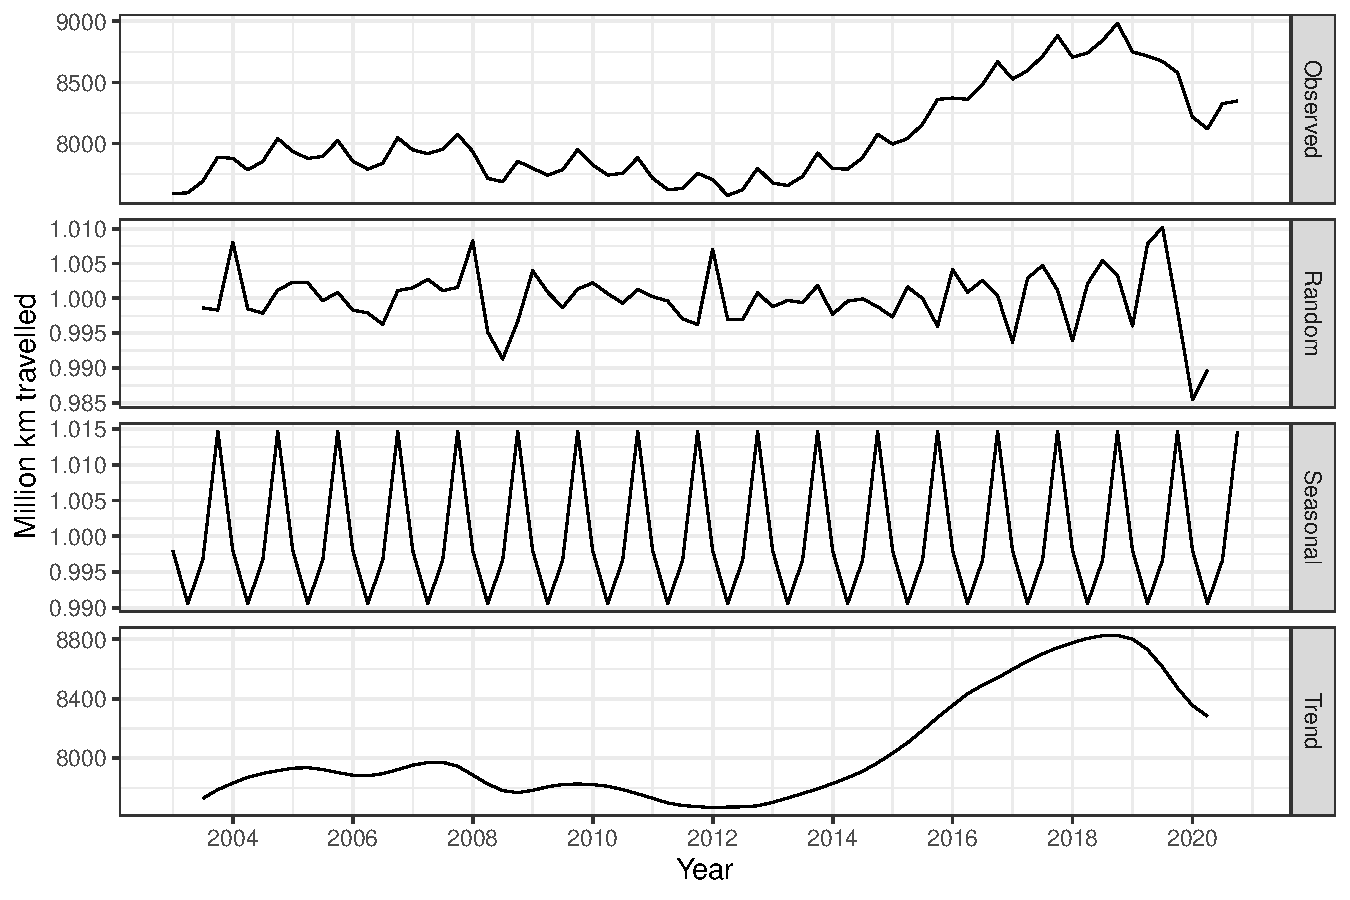
\includegraphics{final_report_files/figure-latex/VKT_ts-1.pdf}
\caption{Decomposition of NZ all regions passenger VKT Time
Series\label{fig:VKT_ts}}
\end{figure}

Figure \ref{fig:VKT_ts} shows the time-series decomposition of the NZ
total VKT data shows a clear seasonal trend, albeit smaller than the
trend from the fuel sales data. There is, however, clearly a large
amount of smoothing going on with this data. This is shown in a couple
of different ways including:

\begin{itemize}
\item The drop of VKT due to lockdown which started in 2020 March is already visible in the data from early 2019. 
\item Related to the previous point, the Random component of Time Series Decomposition shows only a 10\% decrease in VKT spread out over a 1 year period from lockdown, compared to 30\% drop in fuel usage during only 1 quarter shown in the MIBE fuel trade data. 
\item Random variation in MIBE fuel trade data shows around a 3 times greater random variation. There could be a seasonal effect on fuel efficiency which could change the seasonal fuel trend relative to VKT, but there is no reason there would be any significant randomness in fuel efficiency so randomness should be of similar magnitude.
\end{itemize}

This smoothing likely occurs due to the method of VKT data collection
using the odometer readings during WoF/CoF. For a majority of vehicles
WoF is only done once a year and in the case of new cars that could be
up to 3 years. This likely causes the data to show less seasonal trend
than may exist in the real world.

Looking at the long term trend, VKT remained largely flat between 2004
and 2012 after which there was a steady but significant increase until
2019. After this, there is a decrease in VKT due to lockdown, which in
this data set for the above reasons likely started showing its effects
in 2019.

\begin{figure}
\centering
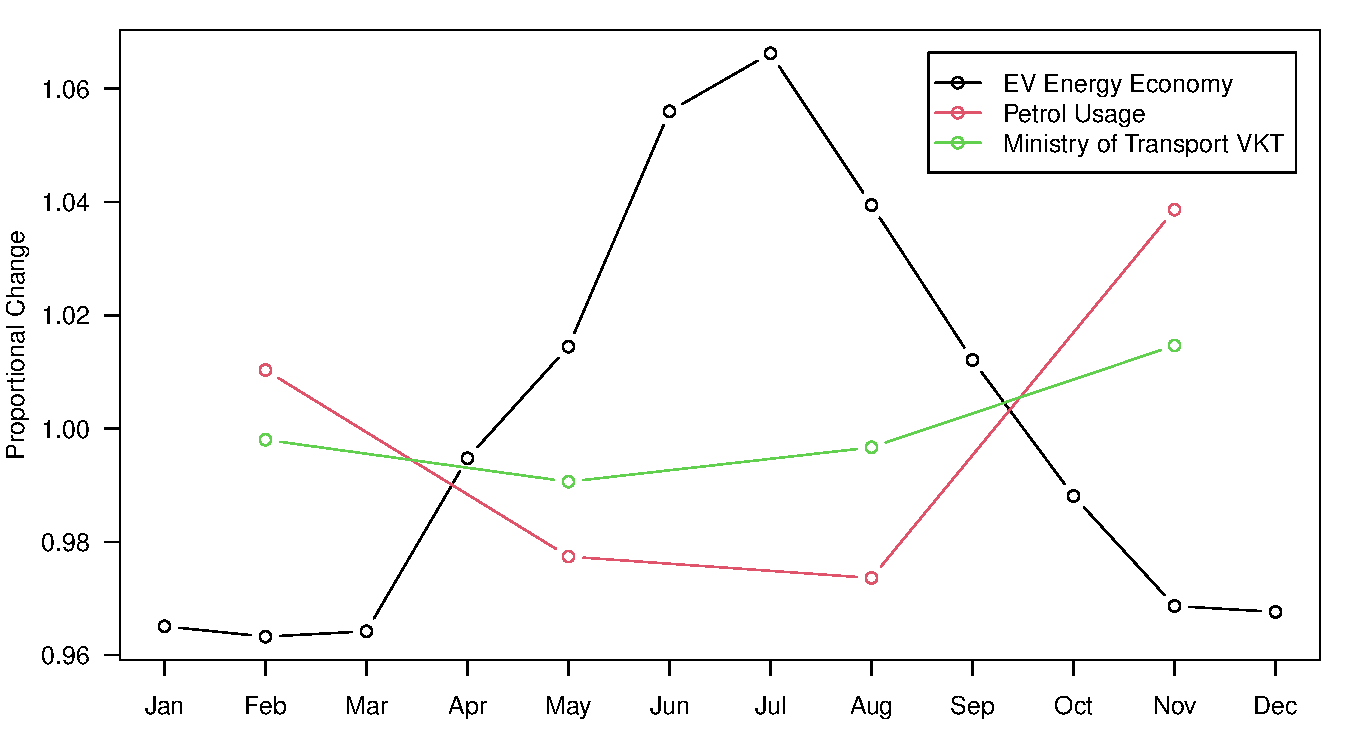
\includegraphics{final_report_files/figure-latex/petrol_VKT_vs_eff-1.pdf}
\caption{NZ Seasonal Component Decompostions}
\end{figure}

Looking at the Seasonal trend of Petrol Usage and VKT data from Ministry
of Transport, we can see an obvious decrease in the winter months with a
peak in the 4th quarter likely corresponding to holiday travel. Petrol
Usage shows this variation to be much larger in the VKT data from
Ministry of Transport. It is unclear whether this would be due to the
smoothing effect as was previously discussed regarding the Ministry of
Transport data, or perhaps a change in efficiency for petrol vehicle by
seasons similar to that of the EV. Combining these 2 data sets it is
reasonable to suggest that in New Zealand, compared to the winter (Q2
and Q3) VKT, the true VKT in the summer (Q1 and Q4) is between 1.3\%
higher, as suggested by the VKT data from Ministry of Transport, to 5\%
higher, according to the petrol usage data.

Looking at the seasonal trend of EV energy economy we can see a much
larger increase in energy economy in the winter months, with average
energy economy in July being 10.7\% higher energy economy than in
February. From the plot we can see that when energy economy of EVs
increases, VKT goes down, suggesting that some increase in total power
usage due to EVs increase in energy economy will be countered by a
decrease in VKT. However, the increase in energy economy is much larger
than the decrease in VKT. This, combined with the fact that winter is
when our electricity grid in New Zealand is already under strain due to
heating demand, suggests that if we ignore the relatively small change
in VKT in our model we can effectively model a worst case scenario. Thus
we propose that monthly distance (\(d_{R}\)) in our model is constant
and determined by the yearly regional VKT data from 2019.

\hypertarget{model}{%
\subsection{Model}\label{model}}

Based on the findings from the data exploration, we propose EV
electricity demand (\(E_{m,R}\)) for each month and region is given by
the formula:

\begin{equation}
\label{eq:energy_usage}
E_{m,R} = \sum_{C} F_C \times \eta_{m,R,C} \times d_{R}
\end{equation}

Where \(F_C\) is the proportion of model in the fleet, \(\eta_{m,R,C}\)
is the montly region energy economy of a particular vehicle model. As
stated in the data exploration section monthly distance (\(d_{R}\)) in
our model is determined from the yearly regional VKT data from 2019 and
has no monthly dependency.

Based on the data exploration we propose we model EV energy economy
(\(\eta_{m,R,C}\)) using a linear model given by the formula:

\begin{equation}
\label{eq:linear_model}
\eta_{m,R,C} = \beta_{CDD}{CDD}_{m,R} + \beta_{HDD}{HDD}_{m,R} + K_R + L_C + \beta_0 + \epsilon
\end{equation}

where \({CDD}_{m,R}\) and \({HDD}_{m,R}\) is the number of CDD and HDD
each month in each region, \(K_R\) is a constant given for each region,
\(L_C\) is a constant given for each model of car and \(\beta_0\) is a
constant intercept. This means \emph{expected} energy economy can be
given by the formula:

\begin{equation}
\label{eq:economy_model}
\eta_{m,R,C} = \beta_{CDD}{CDD}_{m,R} + \beta_{HDD}{HDD}_{m,R} + B_{R,C}
\end{equation}

where \(B_{R,C} = K_R + L_C + \beta_0\) and is effectively a baseline
efficiency of a particular vehicle model is a particular region with no
HDD or CDD.

A different intercept is used for each model of car as a majority of the
variation in efficiency will be due to different vehicle models,
therefore including the vehicle model allows for much better model fit
and smaller confidence intervals. A different intercept is also used for
each weather region as weather might be measured in a cold or hot
section of region and also the region may have more or less hill/highway
which could influence driving patterns impacting efficiency. However the
Gradient of HDD term (\(\beta_{HDD}\)) and CDD term(\(\beta_{CDD}\)) is
kept the same for all regions and models as this is the number we are
trying to find to see how the number of HDD and CDD affect the
efficiency of the EV.

As with the case of the adjusted monthly average power energy economy
(Wh/km) in the linear model a weighting is added to the points in order
to give more weighting to cars with longer distance traveled. This may
give a slight bias towards EVs with proportionally higher highway
mileage. However, from the electricity grids perspective it makes sense
to give less weighting to cars that have traveled 0 or very low km.
Mathematically this means instead of estimating the coefficients by
minimizing the residual sum of squares (RSS) given by the function
\(\sum_{i =1}^{n}(\eta_{i}-\hat{\eta}_{i})^2\) we minimize the function
\(\sum_{i =1}^{n}d \cdot(\eta_{i}-\hat{\eta}_{i})^2\) where \(d\) is the
distance traveled by a car in that month, \(\eta_{i}\) is the actual
power energy economy, and \(\hat{\eta}_{i}\) is the power energy economy
of that vehicle as predicted by the model.

EV energy economy is modelled with a linear model as with the correct
base temperature the usage of power to warm/cool the cabin should be
roughly linear to the HDD/CDD \cite{HDD_est}. This would allow energy
used to heat/cool the car to be isolated for analysis from drivetrain
power energy economy. Conceptually it makes sense that extra power usage
due to heating/cooling demand to be independent from drivetrain demand
as unlike in traditional internal combustion engine (ICE) vehicles where
the energy to heat and cool the cabin comes from the engine, an EVs heat
pump or resistive heater and AC can draw power from the battery
independently of the engine. Unfortunately, this linear correlation may
break down as cars unlike houses or buildings are often only used at
particular hours of the day for short periods so this may break down or
have more dependency towards the temperature at times such as the
morning or evening commute hours.

\begin{longtable}[]{@{}
  >{\raggedright\arraybackslash}p{(\columnwidth - 8\tabcolsep) * \real{0.41}}
  >{\raggedleft\arraybackslash}p{(\columnwidth - 8\tabcolsep) * \real{0.14}}
  >{\raggedleft\arraybackslash}p{(\columnwidth - 8\tabcolsep) * \real{0.16}}
  >{\raggedleft\arraybackslash}p{(\columnwidth - 8\tabcolsep) * \real{0.13}}
  >{\raggedleft\arraybackslash}p{(\columnwidth - 8\tabcolsep) * \real{0.16}}@{}}
\toprule
\begin{minipage}[b]{\linewidth}\raggedright
~
\end{minipage} & \begin{minipage}[b]{\linewidth}\raggedleft
Estimate
\end{minipage} & \begin{minipage}[b]{\linewidth}\raggedleft
Std. Error
\end{minipage} & \begin{minipage}[b]{\linewidth}\raggedleft
t value
\end{minipage} & \begin{minipage}[b]{\linewidth}\raggedleft
Pr(\textgreater\textbar t\textbar)
\end{minipage} \\
\midrule
\endhead
(Intercept) & 132.1 & 0.2867 & 460.8 & 0 \\
HDD & 2.195 & 0.05096 & 43.07 & 0 \\
CDD & 2.347 & 0.5722 & 4.102 & 4.113e-05 \\
Region\_Upper Hutt & -0.4796 & 0.3036 & -1.58 & 0.1141 \\
Region\_Christchurch & -0.9073 & 0.3257 & -2.786 & 0.005348 \\
Region\_Dunedin & 12.06 & 0.3835 & 31.45 & 1.705e-212 \\
Region\_Hamilton & 8.513 & 0.5298 & 16.07 & 8.999e-58 \\
Region\_Nelson & 2.711 & 0.4806 & 5.642 & 1.7e-08 \\
Region\_Rotorua & 5.015 & 0.5462 & 9.182 & 4.597e-20 \\
Region\_Clyde & 4.53 & 0.7491 & 6.048 & 1.494e-09 \\
Region\_Palmerston North & 14.11 & 0.6652 & 21.21 & 6.519e-99 \\
Region\_Stratford & 10.36 & 0.9497 & 10.91 & 1.254e-27 \\
Region\_Napier & 6.316 & 0.8473 & 7.455 & 9.311e-14 \\
Region\_Invercargill & 3.191 & 1.758 & 1.815 & 0.06949 \\
Model\_Nissan Leaf (30 kWh) & 3.401 & 0.2524 & 13.47 & 3.276e-41 \\
Model\_Nissan Leaf (24 kWh) 2011-2012 & 12.39 & 0.3246 & 38.17 &
7.229e-309 \\
Model\_Nissan Leaf (40 kWh) & 10.68 & 0.5174 & 20.63 & 1.046e-93 \\
Model\_Nissan e-NV200 (24 kWh) & 32.71 & 0.5367 & 60.95 & 0 \\
Model\_Hyundai Ioniq (EV) & -18.32 & 0.685 & -26.75 & 3.342e-155 \\
Model\_BMW i3 & -1.335 & 0.7873 & -1.695 & 0.09006 \\
Model\_Hyundai Kona (EV) & 0.6822 & 0.86 & 0.7933 & 0.4276 \\
Model\_Renault Zoe & 11.55 & 0.8507 & 13.57 & 8.383e-42 \\
Model\_Tesla Model 3 & 10.55 & 1.022 & 10.32 & 6.485e-25 \\
Model\_Nissan Leaf (62 kWh) & 25.46 & 1.752 & 14.53 & 1.295e-47 \\
Model\_Kia Niro (EV) & 11.34 & 1.193 & 9.511 & 2.075e-21 \\
Model\_Tesla Model S & 48.38 & 1.69 & 28.63 & 4.806e-177 \\
Model\_Volkswagen e-Golf & 1.208 & 1.538 & 0.7853 & 0.4323 \\
Model\_Tesla Model-X & 104.1 & 1.296 & 80.34 & 0 \\
Model\_Kia Soul & 6.276 & 1.25 & 5.022 & 5.15e-07 \\
Model\_MG ZS EV & 22.12 & 3.9 & 5.671 & 1.439e-08 \\
Model\_Renault Kangoo (van) & 56.63 & 1.537 & 36.84 & 1.301e-288 \\
Model\_Jaguar I-PACE & 73.02 & 2.951 & 24.75 & 1.949e-133 \\
Model\_Peugeot e-208 & 10.96 & 9.581 & 1.144 & 0.2525 \\
\bottomrule
\end{longtable}

\begin{longtable}[]{@{}
  >{\raggedleft\arraybackslash}p{(\columnwidth - 6\tabcolsep) * \real{0.21}}
  >{\raggedleft\arraybackslash}p{(\columnwidth - 6\tabcolsep) * \real{0.31}}
  >{\raggedleft\arraybackslash}p{(\columnwidth - 6\tabcolsep) * \real{0.12}}
  >{\raggedleft\arraybackslash}p{(\columnwidth - 6\tabcolsep) * \real{0.24}}@{}}
\caption{Fitting linear model: economy \textasciitilde{} HDD + CDD +
Region\_ + Model\_}\tabularnewline
\toprule
\begin{minipage}[b]{\linewidth}\raggedleft
Observations
\end{minipage} & \begin{minipage}[b]{\linewidth}\raggedleft
Residual Std. Error
\end{minipage} & \begin{minipage}[b]{\linewidth}\raggedleft
\(R^2\)
\end{minipage} & \begin{minipage}[b]{\linewidth}\raggedleft
Adjusted \(R^2\)
\end{minipage} \\
\midrule
\endfirsthead
\toprule
\begin{minipage}[b]{\linewidth}\raggedleft
Observations
\end{minipage} & \begin{minipage}[b]{\linewidth}\raggedleft
Residual Std. Error
\end{minipage} & \begin{minipage}[b]{\linewidth}\raggedleft
\(R^2\)
\end{minipage} & \begin{minipage}[b]{\linewidth}\raggedleft
Adjusted \(R^2\)
\end{minipage} \\
\midrule
\endhead
22592 & 492.2 & 0.4855 & 0.4848 \\
\bottomrule
\end{longtable}

\hypertarget{how-to-read-this-table}{%
\paragraph{How to read this table:}\label{how-to-read-this-table}}

When computing the linear model as Auckland and Nissan Leaf (24 kWh)
2013-2016 are the most common region and model they are used for the
intercept. In order to get the expected energy economy of a vehicle we
start with the (Intercept) Estimate. We then add to this energy economy
estimate the corresponding region and model Estimate (not needed if it
is Auckland or Nissan Leaf (24 kWh) 2013-2016). Number of HDD per day is
then multiplied by the HDD Estimate from the table and added to the
energy economy estimate. Similarly for CDD days number of CDD per day is
then multiplied by the CDD Estimate from the table and added to this
energy economy estimate.

The HDD term suggests that as the average number of heating degree days
per days increases by 1 the average power energy economy of EVs for the
month increases by 2.19Wh/km. With a p-value of \(<2\times10^{-16}\) we
are quite confident on this value.

The CDD term suggests that as the average number of cooling degree days
per days increases by 1 the average power energy economy of EVs for the
month increases by 2.35Wh/km. With a p-value of \(4.11\times10^{-5}\) we
are less confident on this value. This is likely as there is much less
data in New Zealand regarding cooling degree days.

\begin{figure}
\centering
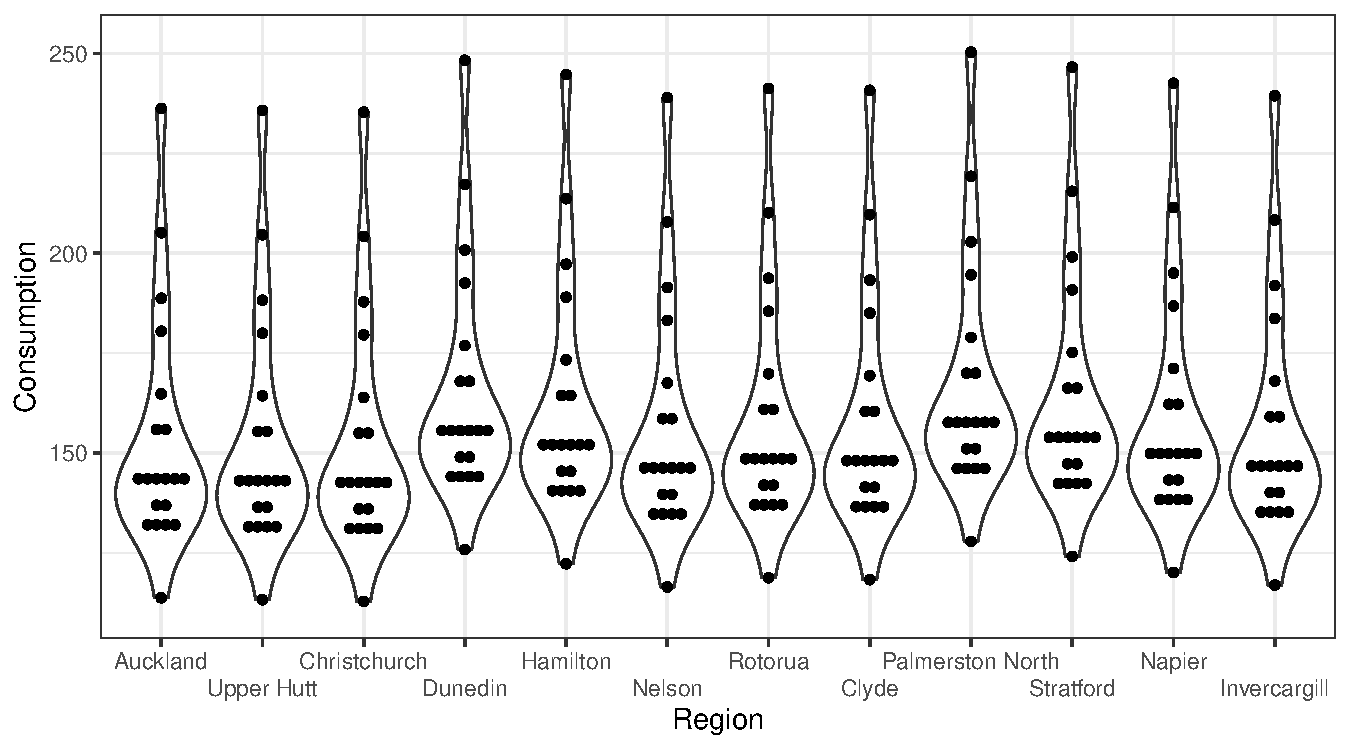
\includegraphics{final_report_files/figure-latex/consum_den-1.pdf}
\caption{distribution of linear model coeffients (effectivly
``baseline'' energy economy by model for each
region)\label{fig:consum_den}}
\end{figure}

\hypertarget{predictions}{%
\subsection{Predictions}\label{predictions}}

We can use the above model to explore future electric vehicle charging
electricity demand. To do this we make the following assumptions:

\begin{itemize}
\item Regional VKT data remains relatively consistent with 2019 VKT data. 2019 is chosen as in NZ there has been a significant increase in VKT in recent years excluding 2020 as there was a significant decrease due to lockdown. As lockdown is an outlier event it would be preferable to not include this in the model so 2019 is used.
\item Regional weather data from 2017 to 2021 remains consistent with future climate of NZ.
\item Flip the Fleet's fleet is representative of NZs future EV fleet (although we explore some extreme cases).
\item Actual VKT of each region remains relatively constant throughout the year.
\end{itemize}

\begin{figure}
\centering
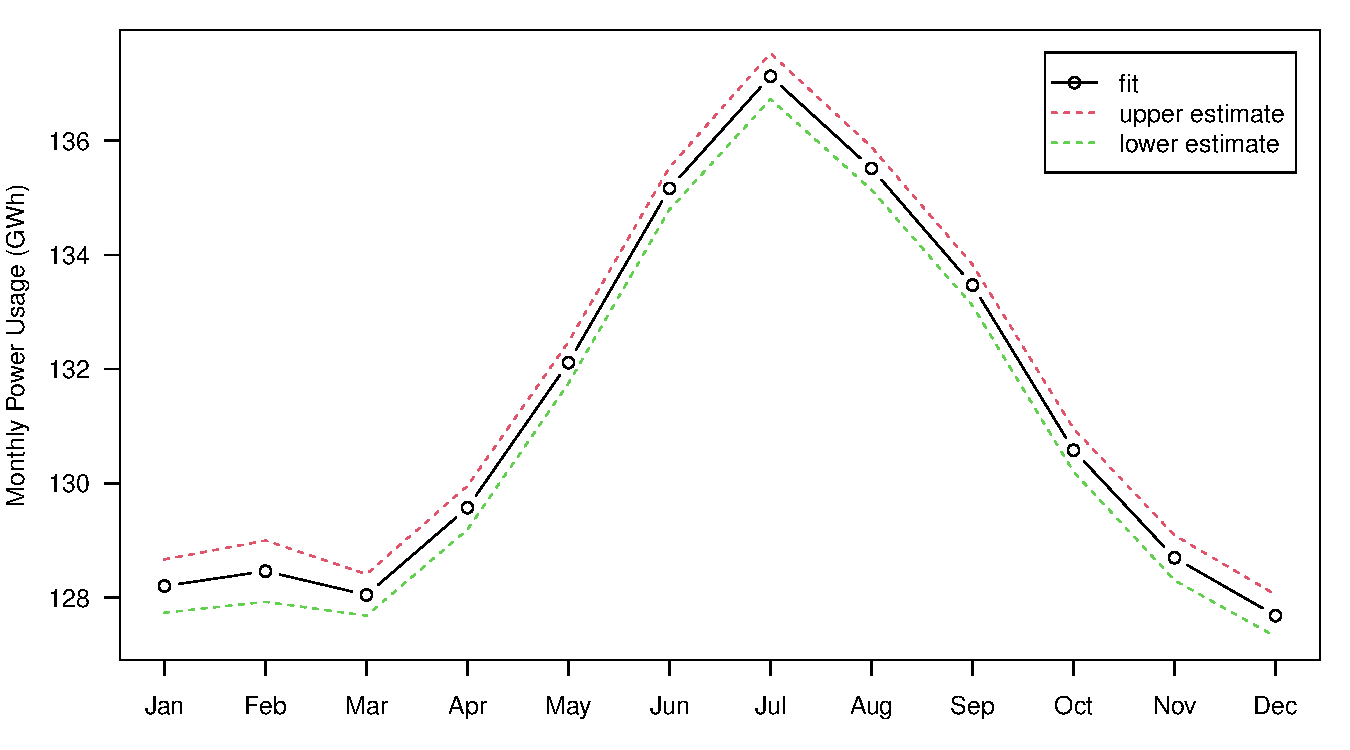
\includegraphics{final_report_files/figure-latex/Auckland_power-1.pdf}
\caption{Auckland region 100\% EV case total EV electricity demand per
month\label{fig:Auckland_power}}
\end{figure}

Combining Auckland only Ministry of Transport 2019 VKT with the energy
economy linear model using Flip the Fleet's vehicle make up and average
weather data from 2017-2021 we can estimate the electricity demand for
100\% EV uptake. This is shown in Figure \ref{fig:Auckland_power}. The
estimated EV electricity demand per month shows a clear seasonal trend
from around 127.7 GWh per month in summer to around 137.1 GWh per month
in the winter.

\begin{figure}
\centering
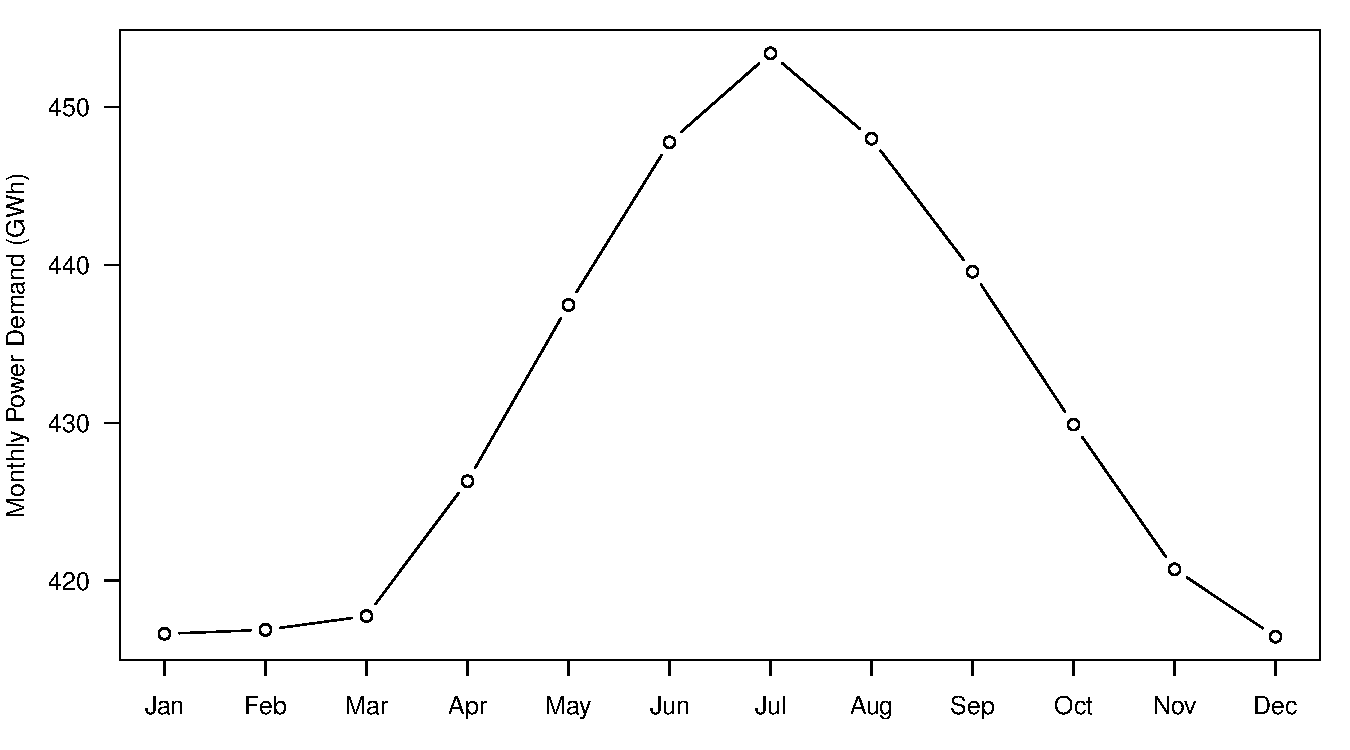
\includegraphics{final_report_files/figure-latex/NZ_power-1.pdf}
\caption{NZ 100\% EV case total EV electricity demand per
month\label{fig:NZ_power}}
\end{figure}

Similarly combining Ministry of Transport 2019 regional VKT with the
energy economy linear model using Flip the Fleets vehicle make up and
average regional weather data from 2017-2021 we can determine the
electricity demand with 100\% EV uptake. This is shown in Figure
\ref{fig:NZ_power} where a clear seasonal trend is observed from around
416 GWh per month in summer to around 453 GWh per month in the winter.

\begin{figure}
\centering
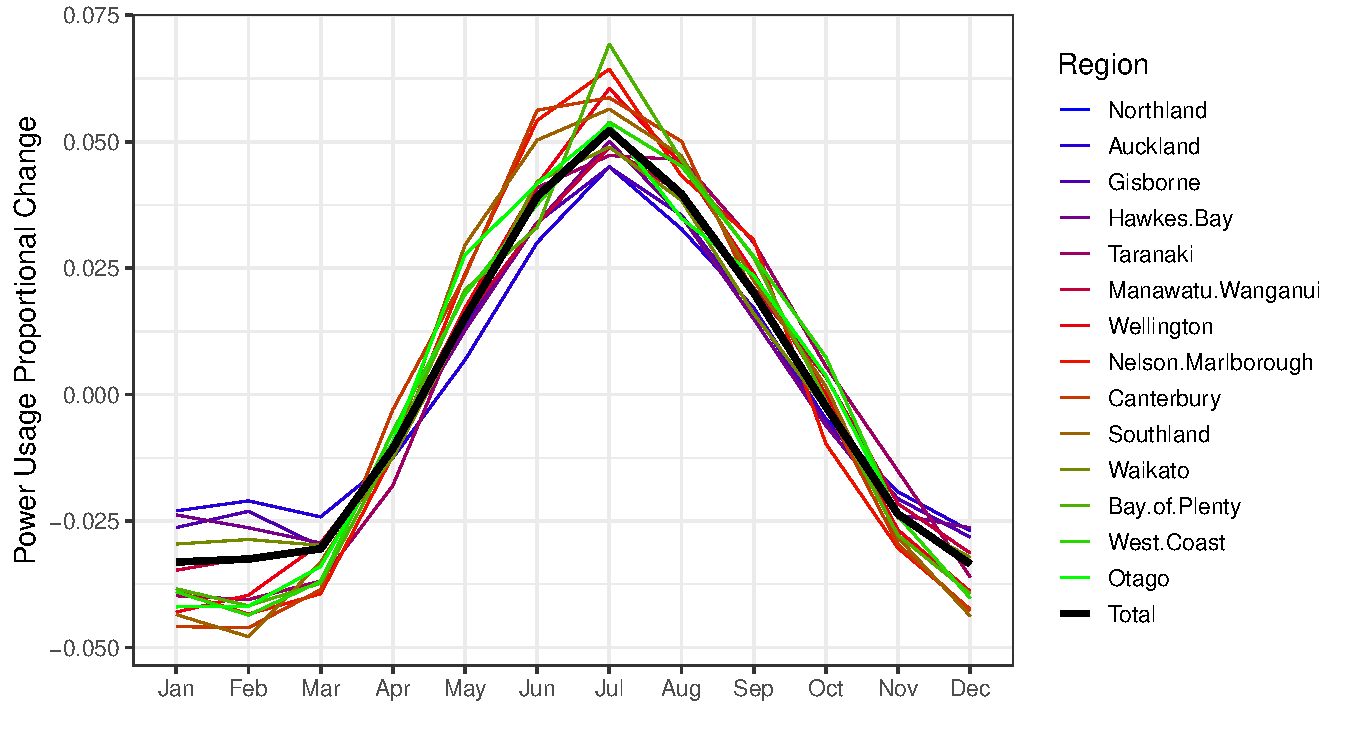
\includegraphics{final_report_files/figure-latex/NZ_region_power_prop-1.pdf}
\caption{All NZ regions monthly proportional change in EV electricity
demand relative to its yearly average\label{fig:NZ_region_power_prop}}
\end{figure}

Applying the same process to all regions we can also plot each regions
proportional change in EV electricity demand relative to its yearly
average. Figure \ref{fig:NZ_region_power_prop} shows all regions follow
a similar seasonal change in power energy economy. Of note, regions like
Northland and Auckland appear to have less of a seasonal trend compared
to regions such as Otago and the West Coast likely due to a warmer
climate leading to increased AC usage during the summer months and
therefore decreasing efficiency in the summer month.

\begin{figure}
\centering
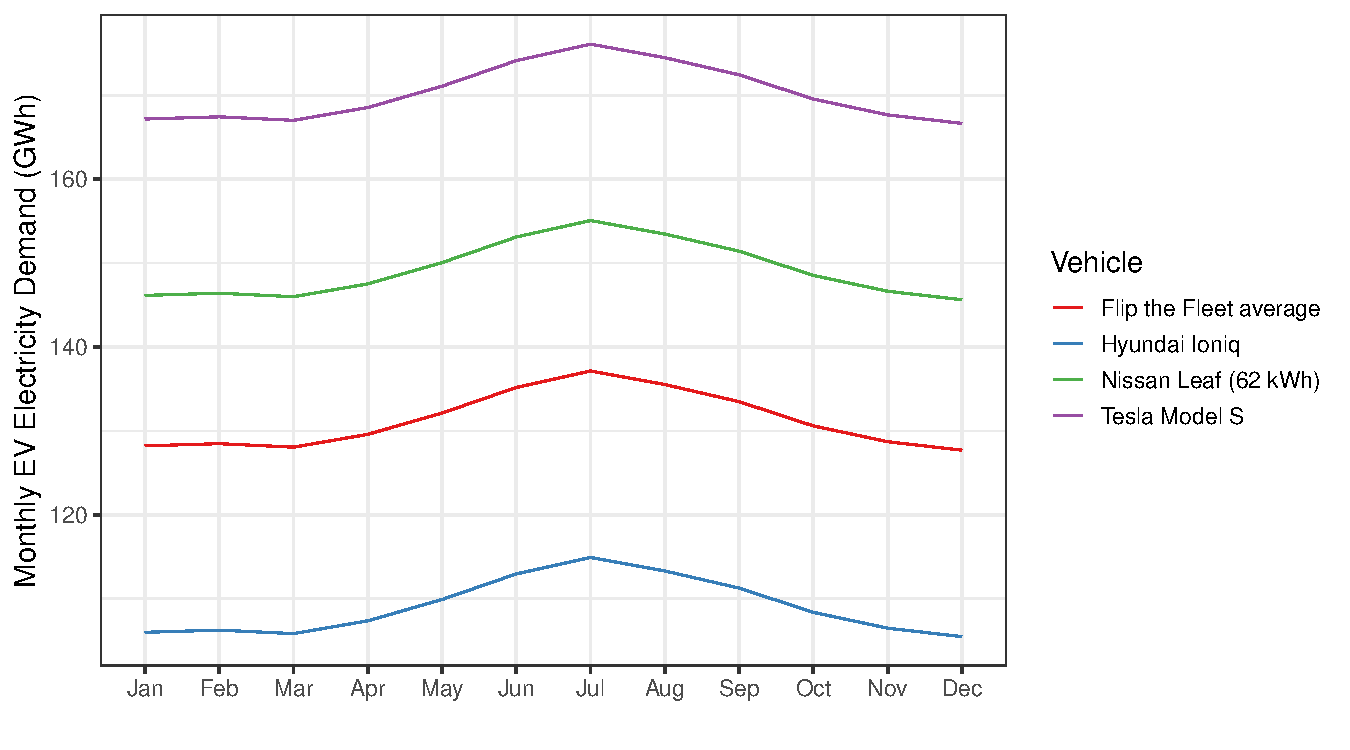
\includegraphics{final_report_files/figure-latex/vehicle_power_usage_auck-1.pdf}
\caption{2019 VKT 100\% EV case Auckland total EV electricity demand
Scenarios by vehicle fleet model
makeup\label{fig:vehicle_power_usage_auck}}
\end{figure}

\begin{figure}
\centering
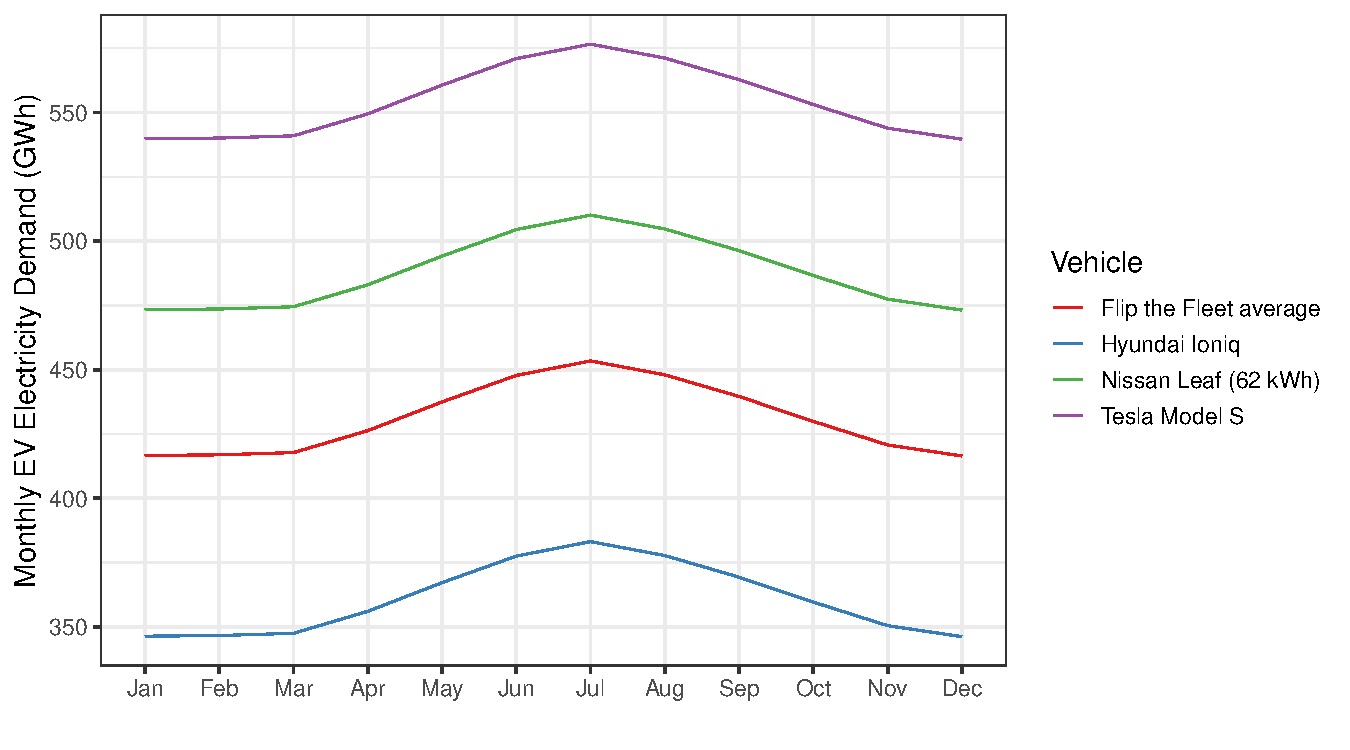
\includegraphics{final_report_files/figure-latex/vehicle_power_usage-1.pdf}
\caption{2019 VKT 100\% EV case NZ total EV electricity demand scenarios
by vehicle fleet model makeup\label{fig:vehicle_power_usage}}
\end{figure}

Combining the regional energy economy used to plot figure
\ref{fig:vehicle_consum} with the 2019 VKT number we can get an expected
EV electricity demand for all of NZ and also for each VKT region. Figure
\ref{fig:vehicle_power_usage} shows with a 100\% EV penetration and an
EV fleet comparable to the Flip the Fleet, the monthly EV electricity
demand for all of NZ goes from 416 GWh minimum in the summer to 453 GWh
maximum EV electricity demand in the winter. If the fleet consisted of
heavier less efficient vehicles like the Tesla Model S this would
increase to 540 GWh minimum in the summer to 577 GWh maximum EV
electricity demand in the winter. Figure
\ref{fig:vehicle_power_usage_auck} shows with a 100\% EV penetration and
an EV fleet comparable to the Flip the Fleet, the monthly EV electricity
demand of Auckland goes from 128 GWh minimum in the summer to 137 GWh
maximum EV electricity demand in the winter. If the fleet consisted of
heavier less efficient vehicles like the Tesla Model S this would
increase to 167 GWh minimum in the summer to 176 GWh maximum EV
electricity demand in the winter.

Figure \ref{fig:vehicle_power_usage} and Figure
\ref{fig:vehicle_power_usage_auck} while showing a seasonal trend, shows
that the vehicle make up of the fleet can have a much greater impact
than anything else on the actual power energy economy that EVs will have
on the power grid.

\hypertarget{comparison-and-incorporation-of-times-model-predictions}{%
\subsubsection{Comparison and Incorporation of Times Model
Predictions}\label{comparison-and-incorporation-of-times-model-predictions}}

To compare our predictions and see how they fit in with other well
established models, ECCA Times Model \cite{times_model} is used as a
comparison. For this, VKT and expected power usage by passenger vehicle
EVs for selected years between 2018 to 2060 was downloaded from EECA.
Expected energy economy (Wh/km) assumed by ECCA was then calculated by
dividing power usage by VKT.

\begin{figure}
\centering
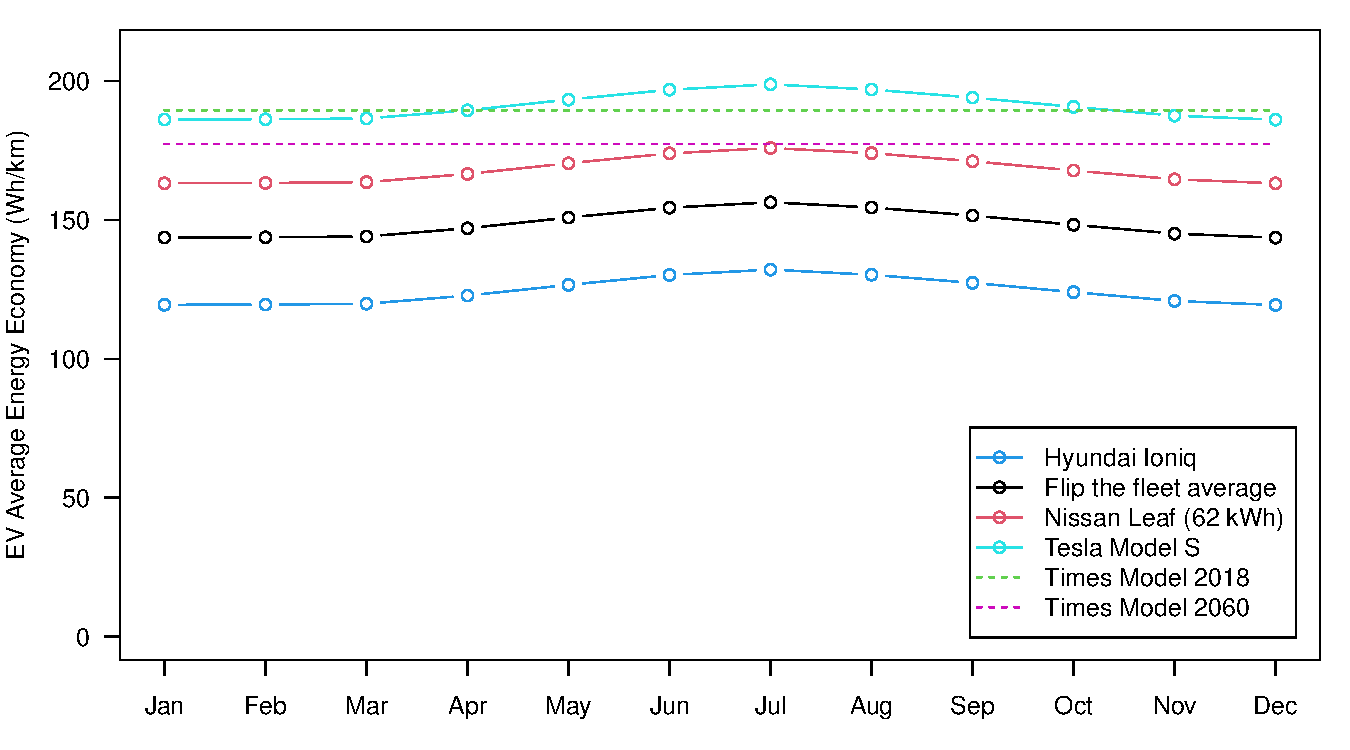
\includegraphics{final_report_files/figure-latex/vehicle_consum-1.pdf}
\caption{NZ vehicle average energy economy
scenarios\label{fig:vehicle_consum}}
\end{figure}

Figure \ref{fig:vehicle_consum} shows comparing flip the fleet energy
economy numbers to EECA's times tui model \cite{times_model} energy
economy we can see that ECCA's times model is based on a much higher
energy economy (lower efficiency) than the flip the fleet data would
suggest. With the energy economy model using the flip the fleet vehicle
make up suggests an average of 148.6Wh/km. However, this is consisting
of primarily of Nissan leafs with 1078 out of 1264 vehicles included in
the flip the fleet data being Nissan leafs which is a quite light and
efficient EV. The 2018 times model energy economy is much more
comparable to much heavier and less efficient Tesla Model S (based on 81
months of efficiency data from 5 vehicles).

\begin{figure}
\centering
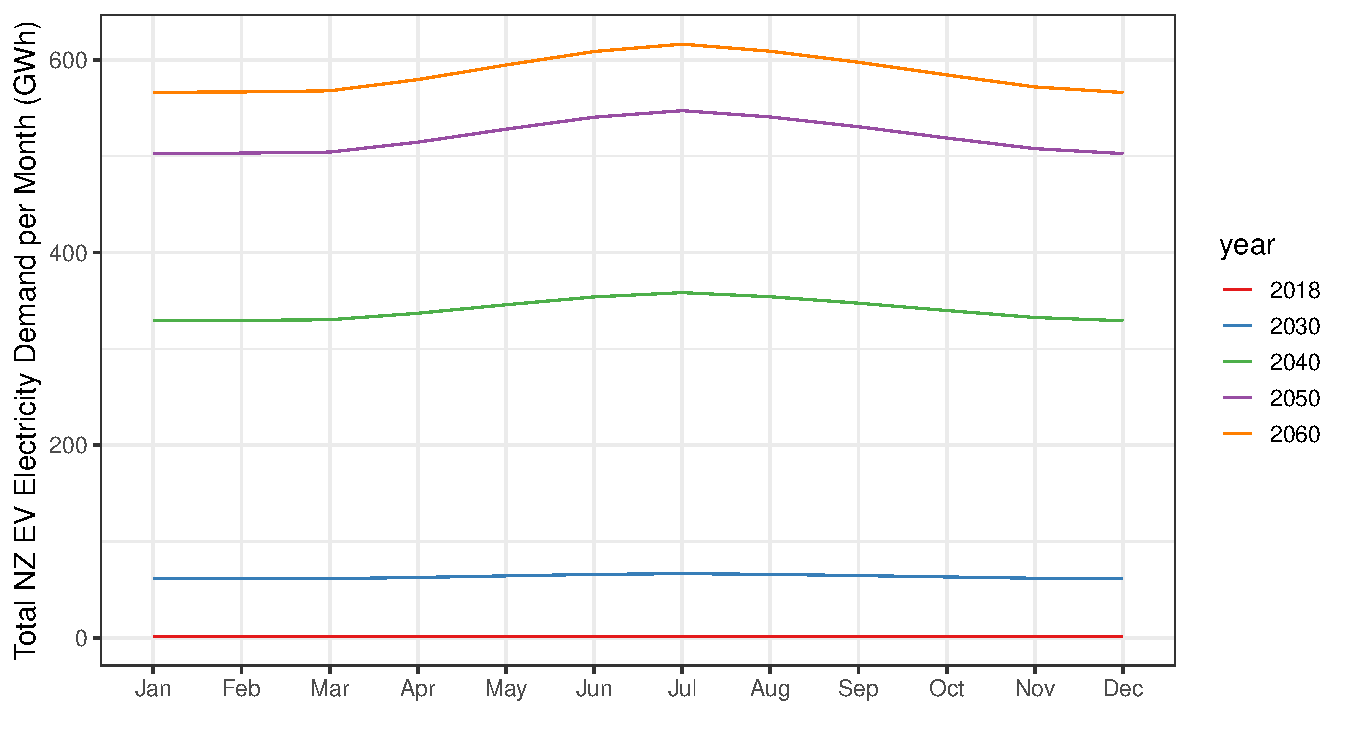
\includegraphics{final_report_files/figure-latex/kea_power_usage-1.pdf}
\caption{NZ EVs electricity demand per month using EECAs Kea VKT and
Flip the Fleets average energy economy\label{fig:kea_power_usage}}
\end{figure}

\begin{figure}
\centering
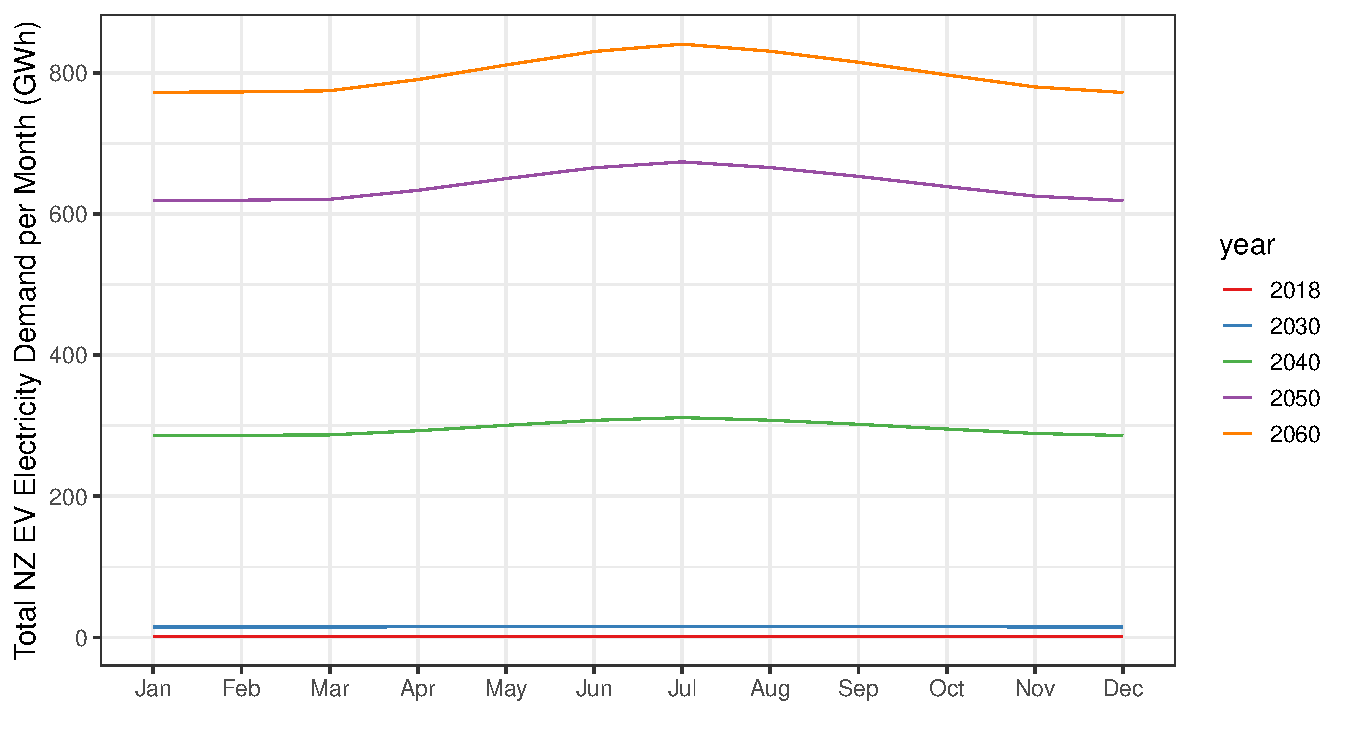
\includegraphics{final_report_files/figure-latex/tui_power_usage-1.pdf}
\caption{NZ EVs electricity demand per month using EECAs Tui VKT and
Flip the Fleets average energy economy\label{fig:tui_power_usage}}
\end{figure}

Figure \ref{fig:kea_power_usage} and Figure \ref{fig:tui_power_usage}
use our energy economy model with Flip the Fleets vehicle make up, NZ
region weather from 2017 to 2021 and Ministry of Transport VKT regional
proportions combined with ECCA times models expected passenger EV VKT to
estimate total monthly power usage of NZ by passenger EVs for select
years between 2018 and 2060.

\begin{thebibliography}{9}
\bibitem{ftf}
\textit{Flip the Fleet Website}
\\\texttt{https://flipthefleet.org/}
\bibitem{ev_range}
\textit{To what degree does temperature impact EV range?}
\\\texttt{\url{https://www.geotab.com/blog/ev-range/}}
\bibitem{ev_highway}
\textit{Why is the range of an EV less on the freeway than the city?}
\\\texttt{\url{https://evcentral.com.au/why-is-the-range-of-an-ev-less-on-the-freeway-than-the-city/}}
\bibitem{fuel_trade}
\textit{MBIE oil trade statistics}
\\\texttt{\url{https://www.mbie.govt.nz/building-and-energy/energy-and-natural-resources/energy-statistics-and-modelling/energy-statistics/oil-statistics/}}
\bibitem{HDD_est}
\textit{Bayesian estimation of a building's base temperature for the calculation of heating degree-days}
\\\texttt{\url{https://www.sciencedirect.com/science/article/abs/pii/S0378778816312907}}
\bibitem{NZTA_VKT}
\textit{Ministry of Transport VKT data website}
\\\texttt{\url{https://www.transport.govt.nz/statistics-and-insights/fleet-statistics/vehicle-kms-travelled-vkt-2/}}
\bibitem{times_model}
\textit{ECCA Times Model}
\\\texttt{\url{https://www.eeca.govt.nz/insights/data-tools/new-zealand-energy-scenarios-times-nz/}}
\end{thebibliography}

\end{document}
